% Provenance (never printed): old terminale S material on mountain ranges and
% continental collision (folds, reverse faults and nappes as signs of
% shortening and thickening; ophiolites and sutures as the trace of a closed
% ocean; the Himalaya and the Alps as examples). Owner (Sync 0): collision,
% fold/anticline/syncline/fold axis, reverse fault/thrust, nappe, ophiolite,
% suture, shortening. Fault is Book 1's (g7), normal fault g11.05's, the root
% and Airy isostasy g11.03's and g12.01's: recalled, never redefined. India's
% past latitudes: figdata/grade-12/india_drift.py (GPlates Web Service, two
% published plate models); shortening: figdata/grade-12/fold_shortening.py;
% the belt map: figdata/grade-12/alpine_belt.py.
\chapter{Building Mountains}\label{ch:g12:mountain-building}

Climbers who reach the top of Mount Everest, \qty{8848.86}{m} above sea
level, stand on limestone. Geologists who brought samples down from
the summit found in them broken pieces of trilobites, ostracods and
crinoids: sea creatures that lived more than 440 million years ago, in the
Ordovician. The highest rock in the world was laid down on the floor of a
sea. This chapter explains how a sea floor ends up on the roof of the world:
two continents collide, and the crust between them is squeezed, folded,
stacked and thickened into a mountain range.
% ledger: sakai05:summit, tulane:roots (marine limestones at the top of Mt. Everest), ics:base.Ordovician, ics:base.Silurian (486.85-443.1 Ma); Book 1: tht:everest (8848.86 m)

\begin{omfigure}
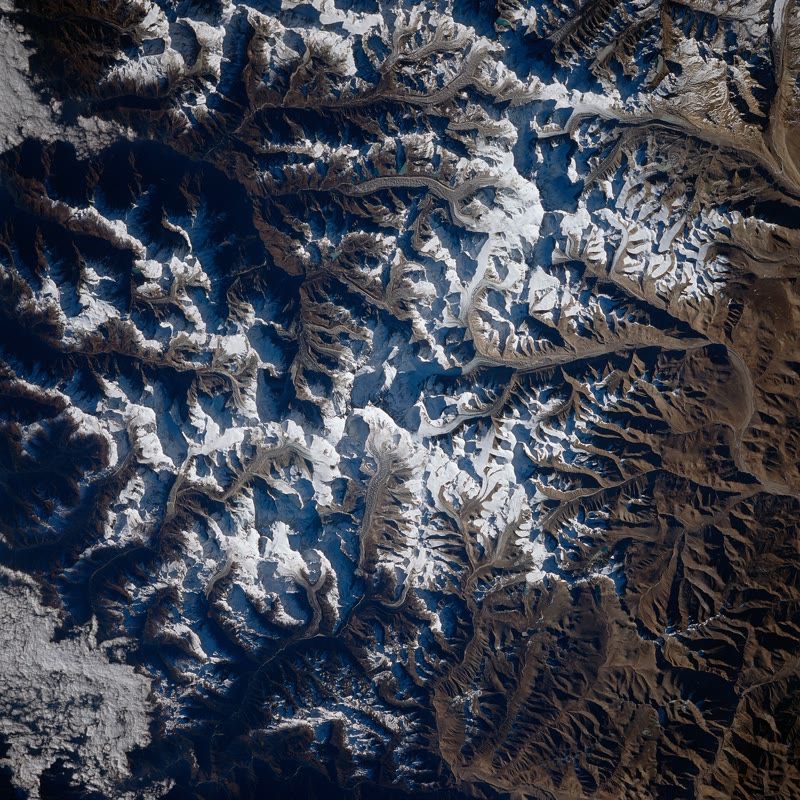
\includegraphics[width=0.5\linewidth]{images/book2/g12-nasa-everest-columbia.jpg}

{\small Mount Everest and many glaciers around it, seen from the space
shuttle Columbia on 30 November 1996. Photograph NASA (public domain).}
\end{omfigure}
% ledger: photo:g12-everest-columbia

\begin{recall}
A plate of \omterm{def:g11:ocean-ridges:oceanic-lithosphere}{oceanic lithosphere}, made at a ridge, sinks back into the mantle
at a trench; its slab pulls it down (\cref{ch:g11:subduction-zones}). The
\omterm{def:g12:continental-crust:continental-crust}{continental crust} is thick and light, about \qty{2830}{kg/m^3} on average
against \qty{3380}{kg/m^3} for the mantle beneath it, so it floats high, and a
thick crust stands higher than a thin one, over a \omterm{def:g12:continental-crust:root}{root}
(\cref{ch:g12:continental-crust,ch:g11:lithosphere-asthenosphere}). A fault
is a break along which the two blocks have moved; at a \omterm{def:g11:ocean-ridges:normal-fault}{normal fault} the
block above the fault plane has moved down, as where the crust is stretched
at a slow ridge (\cref{ch:g11:ocean-ridges}).
\end{recall}
% ledger: cm95:crust, data:prem, tulane:no-subduct, usgs:normal-fault

\section{From subduction to collision}

An ocean that is consumed at a trench faster than it is made at its ridge
shrinks. A continent riding on the sinking plate comes nearer the trench at
the speed of the plate, and in the end it arrives there. The \omterm{def:g11:ocean-ridges:oceanic-lithosphere}{oceanic
lithosphere} ahead of it has gone down; the continent cannot follow it,
because its crust is too light to sink into the denser mantle. \omterm{def:g11:subduction-zones:subduction}{Subduction}
stops. The two continents are squeezed against each other, and the \omterm{def:g11:subduction-zones:slab}{slab}
that hung from the ocean floor eventually breaks off and sinks into the
mantle.
% ledger: earle:collision, tulane:no-subduct

\begin{definition}[Continental collision]\label{def:g12:mountain-building:collision}
A \emph{continental collision}\index{continental collision} is the meeting of
two continents at a convergent plate boundary, once the \omterm{def:g11:ocean-ridges:oceanic-lithosphere}{oceanic lithosphere}
between them has been subducted. Neither continent sinks: the crust between
them is deformed and thickened into a mountain belt.
\end{definition}
% ledger: earle:collision, tulane:no-subduct, usgs:himalaya-collision

\begin{omfigure}
\begin{tikzpicture}[x=0.95cm, y=0.95cm, font=\scriptsize]
  % ---- stage 1: the ocean closes ----
  \begin{scope}[yshift=0cm]
    \fill[omSea] (3.4,0) -- (8.6,0) -- (8.0,-0.5) -- (4.3,-0.5) -- (3.5,0.0) -- cycle;
    \fill[omLithGranite] (0,0.15) -- (3.5,0.15) -- (4.3,-0.5) -- (4.3,-0.75) -- (3.5,-1.0) -- (0,-1.0) -- cycle;
    \fill[omLithBasalt] (4.3,-0.5) -- (8.0,-0.5) .. controls (9.0,-0.75) and (9.6,-1.2) .. (10.4,-2.0)
      -- (10.15,-2.15) .. controls (9.4,-1.4) and (8.9,-1.0) .. (8.0,-0.75) -- (4.3,-0.75) -- cycle;
    \fill[omLithGranite] (8.0,-0.5) -- (8.6,0.2) -- (12,0.2) -- (12,-1.05) -- (9.5,-1.05)
      .. controls (9.0,-0.75) .. (8.0,-0.5) -- cycle;
    \fill[omThm!70] (10.0,0.2) -- (10.3,0.55) -- (10.6,0.2) -- cycle;
    \draw[black!60, line width=0.3pt] (0,0.15) -- (3.5,0.15) -- (4.3,-0.5) -- (8.0,-0.5) -- (8.6,0.2) -- (12,0.2);
    \draw[-{Stealth[length=2mm]}, line width=0.8pt] (1.2,0.45) -- (2.6,0.45);
    \node[anchor=east] at (0,-0.4) {1};
    \node at (1.8,-0.5) {continent};
    \node at (6.1,-0.25) {ocean};
    \node[anchor=north] at (6.1,-0.8) {oceanic lithosphere};
    \node[anchor=south] at (8.0,0.0) {trench};
    \node[anchor=south] at (10.3,0.55) {volcanic arc};
    \node at (11.1,-0.5) {continent};
  \end{scope}
  % ---- stage 2: the continents meet ----
  \begin{scope}[yshift=-3.0cm]
    \fill[omSea] (6.9,0) -- (8.4,0) -- (8.0,-0.4) -- (7.4,-0.35) -- cycle;
    \fill[omLithGranite] (0,0.15) -- (6.8,0.15) -- (7.6,-0.4) -- (8.0,-0.5)
      .. controls (9.0,-0.75) .. (9.5,-1.05) -- (9.2,-1.4) -- (6.5,-1.0) -- (0,-1.0) -- cycle;
    \fill[omLithBasalt] (9.5,-1.05) .. controls (10.0,-1.4) .. (10.6,-2.0) -- (10.35,-2.15)
      .. controls (9.8,-1.6) .. (9.2,-1.4) -- cycle;
    \fill[omLithGranite] (8.0,-0.5) -- (8.6,0.2) -- (12,0.2) -- (12,-1.05) -- (9.5,-1.05)
      .. controls (9.0,-0.75) .. (8.0,-0.5) -- cycle;
    \fill[omLithPeridotite] (7.0,0.15) -- (7.9,0.15) -- (8.3,0.05) -- (7.95,-0.12) -- (7.3,0.0) -- cycle;
    \fill[omThm!70] (10.0,0.2) -- (10.3,0.55) -- (10.6,0.2) -- cycle;
    \draw[-{Stealth[length=2mm]}, line width=0.8pt] (3.2,0.45) -- (4.6,0.45);
    \node[anchor=east] at (0,-0.4) {2};
    \node at (3.4,-0.45) {continent};
    \draw[black!60] (7.6,0.12) -- (7.0,0.75) node[anchor=south east, inner sep=1pt] {slice of ocean floor};
    \node at (11.1,-0.5) {continent};
    \node[anchor=west] at (10.7,-1.9) {slab};
  \end{scope}
  % ---- stage 3: a mountain belt ----
  \begin{scope}[yshift=-6.4cm]
    \fill[omLithGranite] (0,0.15) -- (4.5,0.15) .. controls (6.0,0.4) and (6.6,1.25) .. (7.6,1.3)
      .. controls (8.7,1.3) and (9.6,0.5) .. (10.6,0.2) -- (12,0.2) -- (12,-1.05) -- (10.6,-1.1)
      .. controls (9.5,-2.2) and (8.6,-2.6) .. (7.7,-2.6) .. controls (6.6,-2.6) and (5.6,-1.6) .. (4.5,-1.0)
      -- (0,-1.0) -- cycle;
    \draw[black!60, line width=0.3pt] (0,0.15) -- (4.5,0.15) .. controls (6.0,0.4) and (6.6,1.25) .. (7.6,1.3)
      .. controls (8.7,1.3) and (9.6,0.5) .. (10.6,0.2) -- (12,0.2);
    \draw[black!60, dashed, line width=0.4pt] (0,-1.0) -- (4.5,-1.0) .. controls (5.6,-1.6) and (6.6,-2.6) .. (7.7,-2.6)
      .. controls (8.6,-2.6) and (9.5,-2.2) .. (10.6,-1.1) -- (12,-1.05);
    \draw[omThm, line width=1.0pt] (7.0,1.25) -- (8.3,-2.55);
    \foreach \t in {0.15,0.4,0.65}
      \fill[omLithPeridotite] ($(7.0,1.25)!\t!(8.3,-2.55)$) ++(-0.12,0.05) -- ++(0.3,0) -- ++(-0.05,-0.22) -- ++(-0.3,0) -- cycle;
    \fill[omLithBasalt] (10.9,-1.9) -- (11.5,-2.35) -- (11.35,-2.5) -- (10.75,-2.05) -- cycle;
    \node[anchor=east] at (0,-0.4) {3};
    \node at (2.4,-0.45) {continent};
    \node at (11.3,-0.5) {continent};
    \draw[black!60] (7.2,0.6) -- (5.9,1.5) node[anchor=east, inner sep=1pt] {suture with ophiolites};
    \node at (7.7,-1.9) {root};
    \node[anchor=north] at (11.2,-2.5) {broken-off slab};
    \node[anchor=south] at (7.6,1.35) {mountain belt};
  \end{scope}
\end{tikzpicture}

{\small From \omterm{def:g11:subduction-zones:subduction}{subduction} to collision (not to scale). 1: an ocean closes as
its floor sinks at a trench. 2: the continent arrives at the trench and
cannot sink; slices of ocean floor are pushed onto its edge. 3: the crust
between the two continents is shortened and thickened into a mountain belt
standing over a \omterm{def:g12:continental-crust:root}{root}; the line where the two continents are joined, marked
by slices of ocean floor, is the \omterm{def:g12:mountain-building:suture}{suture}; the \omterm{def:g11:subduction-zones:slab}{slab} breaks off and sinks.}
\end{omfigure}
% ledger: earle:collision, tulane:ocean-basins, usgs:suture, tulane:roots

\subsection{The trace of a vanished ocean}

When the ocean has closed, the two continents are welded along a line.

\begin{definition}[Suture]\label{def:g12:mountain-building:suture}
A \emph{suture}\index{suture} is the line, or narrow zone, along which two
continents have been joined by a collision, once \omterm{def:g11:subduction-zones:subduction}{subduction} between them
has stopped: the trace of a former plate boundary. It marks where the ocean
between them used to be.
\end{definition}
% ledger: usgs:suture, liu20:itsz

What marks a \omterm{def:g12:mountain-building:suture}{suture}? Along many of them lie bodies of rock that belong
nowhere on a continent: from top to bottom, marine sediments, pillow
basalts, a mass of vertical \omterm{def:g11:igneous-rocks:intrusion}{dykes} standing side by side, \omterm{def:g11:ocean-ridges:gabbro}{gabbro}, and at the
base \omterm{def:g11:ocean-ridges:peridotite}{peridotite} of the mantle: the layers of the ocean floor
(\cref{ch:g11:ocean-ridges}), with the top of the mantle beneath them.
% ledger: tulane:ocean-basins

\begin{definition}[Ophiolite]\label{def:g12:mountain-building:ophiolite}
An \emph{ophiolite}\index{ophiolite} is a piece of \omterm{def:g11:ocean-ridges:oceanic-lithosphere}{oceanic lithosphere} ---
sediments, pillow basalts, sheeted \omterm{def:g11:igneous-rocks:intrusion}{dykes}, \omterm{def:g11:ocean-ridges:gabbro}{gabbro} and mantle \omterm{def:g11:ocean-ridges:peridotite}{peridotite} ---
pushed onto \omterm{def:g12:continental-crust:continental-crust}{continental crust}.
\end{definition}
% ledger: tulane:ocean-basins

An \omterm{def:g12:mountain-building:ophiolite}{ophiolite} is stranded ocean floor: a slice of the vanished ocean, pushed
onto a continent instead of sinking with the rest. The mountains raised by
a collision commonly hold some ocean crust and upper mantle, because that is
where an ocean closed. In southern Tibet, \omterm{def:g12:mountain-building:ophiolite}{ophiolites} strung
out along the Indus--Tsangpo \omterm{def:g12:mountain-building:suture}{suture} are remnants of an ocean called the
Neo-Tethys, which lay between India and the region of Lhasa; a \omterm{def:g11:ocean-ridges:gabbro}{gabbro} there
has been dated at 243 million years.
% ledger: tulane:ocean-basins, earle:collision, liu20:itsz

\begin{omfigure}
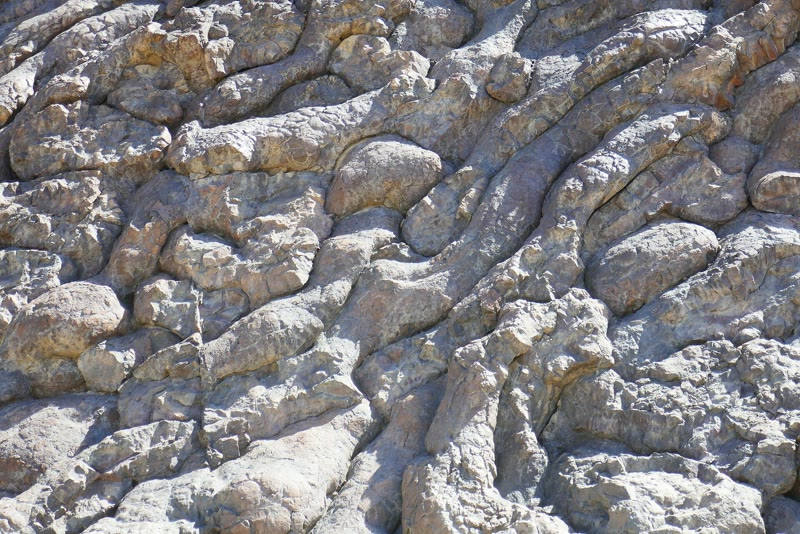
\includegraphics[width=0.6\linewidth]{images/book2/g12-duchoiselle-oman-pillows.jpg}

{\small Pillow lava of the Semail \omterm{def:g12:mountain-building:ophiolite}{ophiolite} at Wadi Jizzi, Oman: lava that
cooled under water as rounded pillows, now on land. Photograph Lionel
Duchoiselle (CC~BY-SA~3.0).}
\end{omfigure}
% ledger: photo:g12-oman-pillows

\section{Shortening the crust}

Squeezed from the sides, a body of rock breaks if it is cold and brittle; if
it is warm enough to behave in a plastic way, it \omterm{def:g12:mountain-building:fold}{folds}. A mountain belt is
full of both \omterm{def:g12:mountain-building:fold}{folds} and faults.
% ledger: earle:folds

\subsection{Folds}

\begin{definition}[Fold; anticline; syncline; fold axis]\label{def:g12:mountain-building:fold}
A \emph{fold}\index{fold} is a bend in layers of rock. Its sloping sides are
the \emph{limbs}; they meet at the \emph{hinge}, where the layers are most
curved, and the line along the hinge is the
\emph{fold axis}\index{fold axis}. An \emph{anticline}\index{anticline} is a fold whose layers bend
upward, its limbs dipping away from the axis; a
\emph{syncline}\index{syncline} is a fold whose layers bend downward, its
limbs dipping toward the axis.
\end{definition}
% ledger: earle:folds, tulane:fold-geometry

The plane through the hinges of the successive layers is the axial plane.
\omterm{def:g12:mountain-building:fold}{Anticlines} and \omterm{def:g12:mountain-building:fold}{synclines} usually come in pairs, the limb of one being the
limb of the next. \omterm{def:g12:mountain-building:fold}{Folds} come in every size, from microscopic to tens of
kilometres across. Once eroded, an \omterm{def:g12:mountain-building:fold}{anticline} shows its oldest layers in
its core and a \omterm{def:g12:mountain-building:fold}{syncline} its youngest; an \omterm{def:g12:mountain-building:fold}{anticline} is not necessarily a
ridge, nor a \omterm{def:g12:mountain-building:fold}{syncline} a valley, because erosion follows the hard and the
soft layers rather than the shape of the \omterm{def:g12:mountain-building:fold}{fold}.
% ledger: earle:folds, tulane:fold-geometry

\begin{omfigure}
\begin{tikzpicture}[x=1.2cm, y=1.2cm, font=\scriptsize]
  \def\W{6}\def\H{2.0}\def\dx{1.35}\def\dy{0.78}
  \tikzset{declare function={zb(\x,\c)=\c+0.8*cos(60*(\x-1.5));}}
  \colorlet{bandA}{omLithSchist!70}\colorlet{bandB}{omLithSand}\colorlet{bandC}{omLithShale}
  \colorlet{bandD}{icsJurassic!35}\colorlet{bandE}{icsTriassic!35}\colorlet{bandF}{icsCretaceous!45}
  % front face
  \begin{scope}
    \clip (0,0) rectangle (\W,\H);
    \fill[bandA] (0,0) rectangle (\W,\H);
    \foreach \c/\col in {0.0/bandB, 0.6/bandC, 1.2/bandD, 1.8/bandE, 2.4/bandF}
      \fill[\col] plot[domain=0:\W, samples=80, smooth] (\x,{zb(\x,\c)}) -- (\W,4) -- (0,4) -- cycle;
    \foreach \c in {0.0,0.6,1.2,1.8,2.4}
      \draw[black!55, line width=0.35pt] plot[domain=0:\W, samples=80, smooth] (\x,{zb(\x,\c)});
  \end{scope}
  % top face: outcrop bands (crossings of the top surface computed for these curves)
  \fill[bandE] (0,\H) -- (0.242,\H) -- ++(\dx,\dy) -- (\dx,\H+\dy) -- cycle;
  \fill[bandD] (0.242,\H) -- (2.758,\H) -- ++(\dx,\dy) -- (0.242+\dx,\H+\dy) -- cycle;
  \fill[bandE] (2.758,\H) -- (3.5,\H) -- ++(\dx,\dy) -- (2.758+\dx,\H+\dy) -- cycle;
  \fill[bandF] (3.5,\H) -- (5.5,\H) -- ++(\dx,\dy) -- (3.5+\dx,\H+\dy) -- cycle;
  \fill[bandE] (5.5,\H) -- (\W,\H) -- ++(\dx,\dy) -- (5.5+\dx,\H+\dy) -- cycle;
  \foreach \x in {0.242,2.758,3.5,5.5} \draw[black!55, line width=0.35pt] (\x,\H) -- ++(\dx,\dy);
  % right face: the layers meet it at constant heights (cylindrical folds)
  \foreach \lo/\hi/\col in {0.0/0.6/bandB, 0.6/1.2/bandC, 1.2/1.8/bandD, 1.8/2.0/bandE}
    \fill[\col] (\W,\lo) -- (\W+\dx,\lo+\dy) -- (\W+\dx,\hi+\dy) -- (\W,\hi) -- cycle;
  \foreach \y in {0.6,1.2,1.8} \draw[black!55, line width=0.35pt] (\W,\y) -- ++(\dx,\dy);
  % outline
  \draw[black, line width=0.5pt] (0,0) rectangle (\W,\H) (0,\H) -- (\dx,\H+\dy) -- (\W+\dx,\H+\dy) -- (\W,\H)
    (\W+\dx,\H+\dy) -- (\W+\dx,\dy) -- (\W,0);
  % fold axes on the top face, axial planes on the front face
  \draw[omThm, line width=1pt] (1.5,\H) -- ++(\dx,\dy);
  \draw[omDef, line width=1pt] (4.5,\H) -- ++(\dx,\dy);
  \draw[omThm, dashed, line width=0.6pt] (1.5,0) -- (1.5,\H);
  \draw[omDef, dashed, line width=0.6pt] (4.5,0) -- (4.5,\H);
  \node[anchor=south, omThm] at (1.5+\dx,\H+\dy) {anticline: fold axis};
  \node[anchor=south, omDef] at (4.5+\dx,\H+\dy) {syncline: fold axis};
  \draw[black!70] (3.2,0.95) -- (3.9,-0.35) node[anchor=north] {limb};
  \draw[black!70] (1.5,1.4) circle (0.07) -- (0.4,-0.35) node[anchor=north] {hinge};
  \draw[black!70] (1.5,0.25) -- (2.0,-0.35) node[anchor=north] {axial plane};
\end{tikzpicture}

{\small An \omterm{def:g12:mountain-building:fold}{anticline} and a \omterm{def:g12:mountain-building:fold}{syncline}, cut by a flat eroded surface (block
diagram, not to scale). The \omterm{def:g12:mountain-building:fold}{fold} axes run along the hinges; the dashed
lines are the traces of the axial planes. On the top surface the eroded
\omterm{def:g12:mountain-building:fold}{anticline} shows older layers in its core, the \omterm{def:g12:mountain-building:fold}{syncline} younger ones.}
\end{omfigure}
% ledger: earle:folds, tulane:fold-geometry

\begin{omfigure}
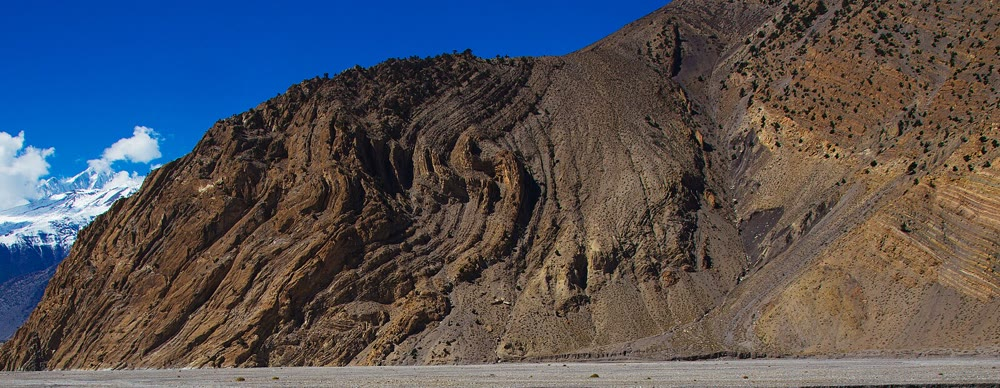
\includegraphics[width=0.95\linewidth]{images/book2/g12-hullot-kali-gandaki-folds.jpg}

{\small Folded layers of rock in a cliff of the Himalaya, about
\qty{3}{km} north-east of Jomsom in the Kali Gandaki gorge, Nepal.
Photograph Jean-Marie Hullot (CC~BY~2.0).}
\end{omfigure}
% ledger: photo:g12-kali-gandaki

The cover of the Varden Hills is folded in the same way, much more gently.
Its sandstone, limestone, shale and chalk were laid down flat, then bent
into an \omterm{def:g12:mountain-building:fold}{anticline} and a \omterm{def:g12:mountain-building:fold}{syncline} whose limbs dip \ang{12}; a later \omterm{def:g11:ocean-ridges:normal-fault}{normal
fault} cuts them.
% ledger: region:name; model in figdata/shared/region.py (LIMB_DIP 12, AXIS_ANTI 3.5 km, AXIS_SYN 7.5 km)

\begin{omfigure}
\begin{tikzpicture}
\begin{axis}[omsection, x=1.25cm, y=0.003125cm, xmin=0, xmax=9.49, ymin=-700, ymax=650,
  xlabel={distance from A (\unit{km})}, ylabel={elevation (\unit{m})},
  ytick={-600,-300,0,300,600}, tick label style={font=\scriptsize}]
\addplot[fill=black!8, draw=black!50, line width=0.3pt, even odd rule] table {figdata/out/shared-region-section-unit-schist.dat};
\addplot[fill=icsTriassic!20, draw=black!50, line width=0.3pt, even odd rule] table {figdata/out/shared-region-section-unit-sandstone.dat};
\addplot[fill=icsJurassic!25, draw=black!50, line width=0.3pt, even odd rule] table {figdata/out/shared-region-section-unit-limestone.dat};
\addplot[fill=icsJurassic!8, draw=black!50, line width=0.3pt, even odd rule] table {figdata/out/shared-region-section-unit-shale.dat};
\addplot[fill=icsCretaceous!20, draw=black!50, line width=0.3pt, even odd rule] table {figdata/out/shared-region-section-unit-chalk.dat};
\addplot[fill=omLithAlluv, draw=black!50, line width=0.3pt, even odd rule] table {figdata/out/shared-region-section-unit-alluvium.dat};
\addplot[black, line width=0.7pt] table {figdata/out/shared-region-section-ground.dat};
\addplot[fault] table {figdata/out/shared-region-section-fault.dat};
% axis positions from figdata/grade-12/fold_shortening.py (section_anticline_km, section_syncline_km; the syncline lies on the hanging wall, shifted by the fault heave)
\draw[omThm, dashed, line width=0.7pt] (axis cs:3.162,-700) -- (axis cs:3.162,660);
\draw[omDef, dashed, line width=0.7pt] (axis cs:7.484,-700) -- (axis cs:7.484,660);
\node[anchor=south, omThm, font=\scriptsize] at (axis cs:3.162,660) {anticline axis};
\node[anchor=south, omDef, font=\scriptsize] at (axis cs:7.484,660) {syncline axis};
\node[anchor=south east, font=\small\bfseries] at (axis cs:0,650) {A};
\node[anchor=south west, font=\small\bfseries] at (axis cs:9.49,650) {B};
\node[font=\scriptsize, fill=white, inner sep=1pt] at (axis cs:1.2,-520) {schist};
\node[font=\scriptsize, fill=white, inner sep=1pt, anchor=east] at (axis cs:6.55,-450) {normal fault};
\end{axis}
\end{tikzpicture}

\smallskip
{\small\tikz\fill[black!8, draw=black!50] (0,0) rectangle (0.35,0.22);~schist \quad
\tikz\fill[icsTriassic!20, draw=black!50] (0,0) rectangle (0.35,0.22);~sandstone \quad
\tikz\fill[icsJurassic!25, draw=black!50] (0,0) rectangle (0.35,0.22);~limestone \quad
\tikz\fill[icsJurassic!8, draw=black!50] (0,0) rectangle (0.35,0.22);~shale \quad
\tikz\fill[icsCretaceous!20, draw=black!50] (0,0) rectangle (0.35,0.22);~chalk \quad
\omve{2.5}}

{\small Section A--B across the Varden Hills, from the south-west to the
north-east. The cover rests on the schist basement and is folded into an
\omterm{def:g12:mountain-building:fold}{anticline} and a \omterm{def:g12:mountain-building:fold}{syncline}; the \omterm{def:g11:ocean-ridges:normal-fault}{normal fault}, younger than the \omterm{def:g12:mountain-building:fold}{folds}, drops
the north-eastern block. The vertical scale is stretched 2.5 times, which
makes the limbs look steeper than they are. Data: the series' model of the
region.}
\end{omfigure}
% ledger: region:name; computed in figdata/shared/region.py (section A-B)

\subsection{Reverse faults, thrusts and nappes}

Where the crust is squeezed while cold and brittle, it breaks along faults
of another kind than the \omterm{def:g11:ocean-ridges:normal-fault}{normal faults} of stretched crust.

\begin{definition}[Reverse fault; thrust]\label{def:g12:mountain-building:thrust}
A \emph{reverse fault}\index{reverse fault} is an inclined fault along which
the block above the fault plane has moved up relative to the block below
it. Reverse faults form where the crust is squeezed. A
\emph{thrust}\index{thrust} is a reverse fault with a gentle dip, less than
\ang{45}.
\end{definition}
% ledger: earle:reverse-thrust, tulane:fold-geometry

A \omterm{def:g12:mountain-building:thrust}{thrust} can carry a sheet of rock for tens of kilometres, and then older
rocks come to rest on top of younger ones, against the order in which they
were laid down. In the Rocky Mountains, the McConnell Thrust has pushed a
pile of sedimentary rocks about \qty{800}{m} thick some \qty{40}{km} from
west to east: limestone about 500 million years old now lies on a mudstone
about 75 million years old.
% ledger: earle:reverse-thrust

\begin{definition}[Nappe]\label{def:g12:mountain-building:nappe}
A \emph{nappe}\index{nappe} is a large sheet of rock that has been carried a
long distance, often tens of kilometres, over the rocks beneath it along a
\omterm{def:g12:mountain-building:thrust}{thrust} that is nearly flat.
\end{definition}
% ledger: ngu:nappe, earle:reverse-thrust

A \omterm{def:g12:mountain-building:nappe}{nappe} can carry rocks that formed far away, even slices of ocean floor; it
can itself be folded, its layers overturned. Mountain belts pile up \omterm{def:g12:mountain-building:nappe}{nappes}
one on top of another. Erosion later cuts holes through a \omterm{def:g12:mountain-building:nappe}{nappe}, opening
windows onto the rocks below, and leaves isolated pieces of it standing on
the younger rocks.
% ledger: ngu:nappe

\begin{omfigure}
\begin{tikzpicture}[x=1.0cm, y=1.0cm, font=\scriptsize]
  % rocks in place (younger), flat-lying
  \fill[icsCretaceous!25] (0,-1.6) rectangle (12,-0.4);
  \fill[icsJurassic!25] (0,-1.6) rectangle (12,-1.1);
  \draw[black!50, line width=0.3pt] (0,-1.1) -- (12,-1.1);
  \fill[white] (5.6,-0.4) -- (6.2,-0.62) -- (6.8,-0.4) -- cycle;
  % the nappe (older rocks) above a nearly flat thrust, cut by erosion
  \fill[omLithSchist!80] (0.8,-0.4) .. controls (1.2,0.35) and (1.9,0.35) .. (2.3,-0.4) -- cycle;
  \fill[omLithSchist!80] (3.2,-0.4) .. controls (3.9,0.9) and (4.8,0.9) .. (5.6,-0.4) -- cycle;
  \fill[omLithSchist!80] (6.8,-0.4) .. controls (7.1,0.9) and (7.7,1.3) .. (8.4,1.25) -- (12,0.9) -- (12,-0.4) -- cycle;
  % ground surface
  \draw[black, line width=0.6pt] (0,-0.4) -- (0.8,-0.4) .. controls (1.2,0.35) and (1.9,0.35) .. (2.3,-0.4)
     -- (3.2,-0.4) .. controls (3.9,0.9) and (4.8,0.9) .. (5.6,-0.4) -- (6.2,-0.62) -- (6.8,-0.4)
     .. controls (7.1,0.9) and (7.7,1.3) .. (8.4,1.25) -- (12,0.9);
  % thrust traces (teeth on the block that moved over)
  \draw[thrust fault] (0.8,-0.4) -- (2.3,-0.4);
  \draw[thrust fault] (3.2,-0.4) -- (5.6,-0.4);
  \draw[thrust fault] (6.8,-0.4) -- (12,-0.4);
  \draw[-{Stealth[length=2mm]}, line width=0.9pt] (11.4,1.45) -- (9.6,1.6);
  \node[anchor=south] at (10.5,1.55) {motion of the nappe};
  \node at (9.9,0.3) {nappe: older rocks};
  \node[fill=white, inner sep=1pt] at (2.0,-0.85) {rocks in place: younger};
  \draw[black!60] (1.55,0.0) -- (1.3,0.8) node[anchor=south] {isolated piece};
  \draw[black!60] (6.2,-0.58) -- (6.2,-0.68) node[anchor=north, fill=white, inner sep=1pt] {window};
  \draw[black!60] (9.0,-0.42) -- (9.3,-0.68) node[anchor=north, fill=white, inner sep=1pt] {thrust};
\end{tikzpicture}

{\small A \omterm{def:g12:mountain-building:nappe}{nappe} (not to scale): a sheet of older rocks carried along a
nearly flat \omterm{def:g12:mountain-building:thrust}{thrust} over younger rocks that have stayed in place. Erosion has
cut a window through it and left an isolated piece of it on the left. The
teeth on the \omterm{def:g12:mountain-building:thrust}{thrust} point toward the block that moved over.}
\end{omfigure}
% ledger: ngu:nappe, earle:reverse-thrust

\begin{omfigure}
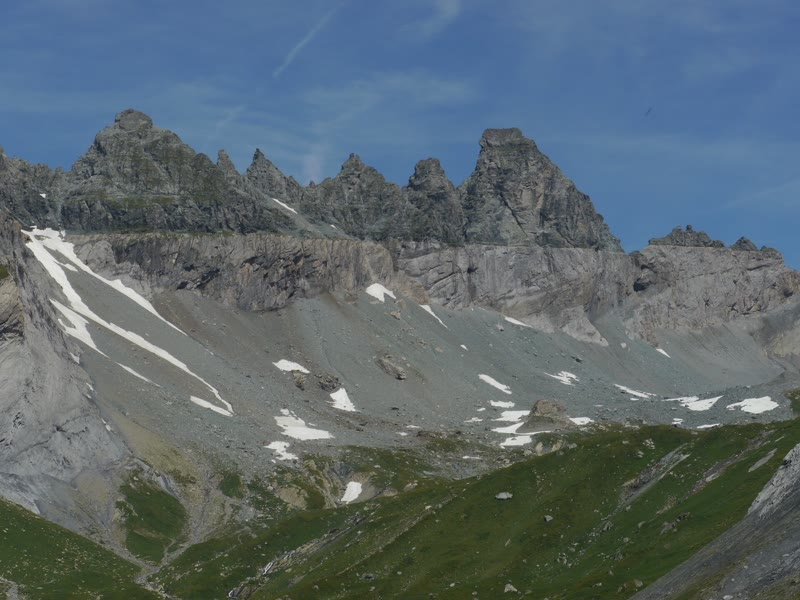
\includegraphics[width=0.5\linewidth]{images/book2/g12-heine-glarus-thrust.jpg}

{\small The Glarus Thrust in the Alps of eastern Switzerland. The dark
rocks of the peaks, laid down in the Permian, between about 299 and 252
million years ago, rest on lighter and much younger rocks; the \omterm{def:g12:mountain-building:thrust}{thrust} is the
sharp boundary between them. The upper rocks have moved some 40 to
\qty{50}{km}. Photograph Christian Heine (CC~BY-SA~3.0).}
\end{omfigure}
% ledger: photo:g12-glarus (Verrucano, Permian; displacement 40-50 km, Pfiffner 1985), ics:base.Permian, ics:base.Triassic

\subsection{Measuring the shortening}

\omterm{def:g12:mountain-building:fold}{Folds} and \omterm{def:g12:mountain-building:thrust}{thrusts} both make the crust shorter in the direction it is
squeezed.

\begin{definition}[Shortening]\label{def:g12:mountain-building:shortening}
The \emph{shortening}\index{shortening} of a layer is the fraction of its
length that it has lost: if it was $L_0$ long and now spans $L$,
\[
  e = \frac{L_0 - L}{L_0}.
\]
\end{definition}

To measure it, one needs the original length $L_0$. In many \omterm{def:g12:mountain-building:fold}{folds} the
layers keep their thickness as they bend, sliding over one another like the
pages of a bent book; such a layer is not stretched along its length. This
gives the original length.
% ledger: tulane:fold-geometry (flexural folds keep their thickness)

\begin{proposition}[The shortening of a folded layer]\label{prop:g12:mountain-building:shortening}
If a layer has folded without being stretched or squeezed along itself,
its original length $L_0$ is its length measured along the folded layer.
For a \omterm{def:g12:mountain-building:fold}{fold} with straight limbs dipping at an angle $\theta$,
\[
  e = 1 - \cos\theta .
\]
\end{proposition}

\begin{proof}
Unfolding the layer, without stretching it, lays it out flat with its
length unchanged; so $L_0$ is the length along the layer. On a straight
limb of length $\ell$ dipping at $\theta$, the horizontal distance covered
is $\ell\cos\theta$ (right triangle). Adding all the limbs, the layer of
length $L_0$ spans $L = L_0\cos\theta$, and $e = (L_0 - L_0\cos\theta)/L_0 =
1 - \cos\theta$.
\end{proof}

\begin{omfigure}
\begin{tikzpicture}
\begin{axis}[name=sine, x=2.0cm, y=2.0cm, axis lines=none,
  xmin=-0.05, xmax=2.25, ymin=-0.4, ymax=0.8, clip=false]
% computed in figdata/grade-12/fold_shortening.py (part sine: A/lambda = 0.25, e = 31.7 %)
\addplot[omLithSand!80!black, line width=1.6pt] table[x=x, y=y] {figdata/out/grade-12-fold_shortening-sine.dat};
\draw[omThm, line width=1.6pt] (axis cs:0,0.62) -- (axis cs:2.196,0.62);
\draw[black!60, |-|] (axis cs:0,-0.32) -- node[below, font=\scriptsize] {$L$ (today)} (axis cs:1.5,-0.32);
\node[anchor=south west, font=\scriptsize, omThm] at (axis cs:0,0.64) {$L_0$: the same layer unfolded};
\end{axis}
\begin{axis}[omrecord, at={(sine.east)}, anchor=west, xshift=1.4cm, width=0.46\linewidth, height=4.6cm,
  xmin=0, xmax=80, ymin=0, ymax=85, xlabel={limb dip $\theta$ (\unit{\degree})},
  ylabel={shortening $e$ (\unit{\percent})}, xtick={0,20,...,80}]
% computed in figdata/grade-12/fold_shortening.py (part dip: e = 1 - cos theta)
\addplot[omProp, line width=1pt] table[x=theta, y=e_pct] {figdata/out/grade-12-fold_shortening-dip.dat};
\addplot[only marks, mark=*, mark size=1.6pt, omThm] coordinates {(12,2.185) (30,13.397) (60,50)};
\node[anchor=south, font=\scriptsize, align=center] at (axis cs:12,6) {Varden:\\\qty{2.2}{\percent}};
\node[anchor=west, font=\scriptsize] at (axis cs:32,10) {\qty{13}{\percent}};
\node[anchor=south east, font=\scriptsize] at (axis cs:60,51) {\qty{50}{\percent}};
\end{axis}
\end{tikzpicture}

{\small Left: a folded layer spans $L$; laid out flat, without being
stretched, it is $L_0$ long (here the \omterm{def:g12:mountain-building:fold}{folds} are as high as a quarter of
their wavelength, and $L$ is \qty{68}{\percent} of $L_0$). Right: the
\omterm{def:g12:mountain-building:shortening}{shortening} of a \omterm{def:g12:mountain-building:fold}{fold} with straight limbs, $1 - \cos\theta$, against the dip
of its limbs. Gentle \omterm{def:g12:mountain-building:fold}{folds} shorten a layer very little.}
\end{omfigure}
% values: sine_025_e_pct 31.68 (L/L0 = 0.683); varden_e_pct 2.1852; chevron_30 13.397; chevron_60 50 (fold_shortening.py)

\begin{method}[Measuring the shortening on a cross-section]\label{met:g12:mountain-building:shortening}
\begin{enumerate}
  \item Check that the section is drawn at true scale. If its vertical scale
        is stretched, dips and lengths along the layers are too large: redraw
        it, or correct each dip first.
  \item Choose one layer boundary that can be followed across the section;
        where a fault cuts it, join the two cut ends as they were before the
        fault moved.
  \item Measure its length along the layer, $L_0$: follow it with a thread,
        or add up short straight pieces.
  \item Measure the horizontal distance between its two ends, $L$.
  \item Compute $e = (L_0 - L)/L_0$; for straight limbs of known dip,
        $e = 1 - \cos\theta$ gives it at once.
\end{enumerate}
\end{method}

\begin{example}[The Varden folds]\label{ex:g12:mountain-building:varden}
The limbs of the Varden \omterm{def:g12:mountain-building:fold}{folds} dip \ang{12}, so the cover was shortened by
$e = 1 - \cos\ang{12} = 1 - 0.978 = 0.022$, about \qty{2.2}{\percent}: a
stretch of the region \qty{10}{km} wide today was $10/\cos\ang{12} \approx
\qty{10.22}{km}$ wide before folding. Measured on section A--B as drawn, the
limbs would look about \ang{28} steep, because the vertical scale is
stretched 2.5 times: $\tan\theta$ is multiplied by 2.5, and $\arctan(2.5
\tan\ang{12}) \approx \ang{28}$. Read at face value, that would give a
\omterm{def:g12:mountain-building:shortening}{shortening} of \qty{12}{\percent}, more than five times too much.
\end{example}
% values: varden_e_pct 2.1852, varden_L0_for_10km 10.223 (fold_shortening.py); arctan(2.5 x 0.2126) = 27.98 deg; 1 - cos 27.98 = 0.117

Gentle \omterm{def:g12:mountain-building:fold}{folds} absorb little. A tightly folded belt, with limbs dipping
\ang{60}, has been shortened by half; and a single nearly flat \omterm{def:g12:mountain-building:thrust}{thrust} that
has carried a \omterm{def:g12:mountain-building:nappe}{nappe} \qty{40}{km} absorbs \qty{40}{km} of \omterm{def:g12:mountain-building:shortening}{shortening}, as much
as a very wide belt of gentle \omterm{def:g12:mountain-building:fold}{folds}.

\section{Thickening and uplift}

\omterm{def:g12:mountain-building:shortening}{Shortening} does not destroy rock. A strip of crust squeezed to a fraction of
its former width keeps its volume, so it must grow thicker: if a crust
$H_0$ thick is shortened from a width $L_0$ to $L$ along the whole length of
the belt, its cross-section keeps its area, $H L = H_0 L_0$, and
\[
  H = H_0\,\frac{L_0}{L} = \frac{H_0}{1 - e}.
\]
A crust \qty{35}{km} thick shortened by \qty{50}{\percent} becomes
\qty{70}{km} thick. Then \omterm{def:g11:lithosphere-asthenosphere:isostasy}{isostasy} does the rest: a thicker crust floats
higher, over a deeper \omterm{def:g12:continental-crust:root}{root} (\cref{prop:g11:lithosphere-asthenosphere:airy}).
With Airy's model and the densities of the recall, a crust thicker by
$\Delta H$ stands higher by $\Delta H\,(\rho_m - \rho_c)/\rho_m = \Delta H
\times 550/3380$, about a sixth of the extra thickness; the other five
sixths form the \omterm{def:g12:continental-crust:root}{root}. The crust is \num{35} to \qty{40}{km} thick away from
mountain belts, and 50 to \qty{70}{km} thick beneath them: the higher the
mountains, the thicker the crust.
% ledger: tulane:roots, cm95:crust, data:prem

This is how sea-floor limestone came to the top of Everest: laid down on the
floor of a sea, it was carried north with India, stacked in the \omterm{def:g12:mountain-building:thrust}{thrust}
sheets of the Himalaya, and lifted as the crust beneath it thickened and
rose. Such a vertical movement of the crust is called uplift.
% ledger: sakai05:summit, sakai05:stacking, tulane:roots (uplift), usgs:himalaya-collision

\section{Two ranges}

\subsection{The Himalaya}

The Himalaya stretch \qty{2900}{km} along the border between India and
Tibet. About 80 million years ago India lay roughly \qty{6400}{km} south of
Asia, across an ocean, and moved north at about \qty{9}{cm} a year; it met
Asia between 40 and 50 million years ago, and its northward advance then
slowed. Plate reconstructions show the journey in detail: built from many
kinds of evidence, among them the tracks of hotspots
(\cref{ch:g11:plate-motions}), they move the plates back in time step by
step.
% ledger: usgs:himalaya-collision, muller19:frame, muller22:frame

\begin{omfigure}
\begin{tikzpicture}
\begin{axis}[omrecord, omage, name=lat, width=0.5\linewidth, height=5.2cm,
  xmin=0, xmax=100, ymin=-45, ymax=35, xlabel={age (\unit{Ma})}, ylabel={latitude (\unit{\degree})},
  xtick={0,20,...,100}, ytick={-40,-20,...,40},
  legend style={font=\scriptsize, at={(0.98,0.03)}, anchor=south east, fill=white}]
% computed in figdata/grade-12/india_drift.py (part lat; GPlates Web Service, MULLER2022 and MULLER2019)
\fill[omThm!12] (axis cs:40,-45) rectangle (axis cs:50,35);
\addplot[omThm, line width=1.1pt] table[x=age, y=m22_india] {figdata/out/grade-12-india_drift-lat.dat};
\addplot[omThm, dashed, line width=0.8pt] table[x=age, y=m19_india] {figdata/out/grade-12-india_drift-lat.dat};
\addplot[omDef, line width=1.1pt] table[x=age, y=m22_lhasa] {figdata/out/grade-12-india_drift-lat.dat};
\addplot[black!50, line width=0.4pt, forget plot] coordinates {(0,0) (100,0)};
\legend{{central India (2022)}, {central India (2019)}, {Lhasa (2022)}}
\end{axis}
\begin{axis}[omrecord, omage, at={(lat.east)}, anchor=west, xshift=1.9cm, width=0.42\linewidth, height=5.2cm,
  xmin=0, xmax=100, ymin=0, ymax=160, xlabel={age (\unit{Ma})},
  ylabel={northward speed (\unit{mm/yr})}, xtick={0,20,...,100}]
% computed in figdata/grade-12/india_drift.py (part steps: 5-Myr steps)
\fill[omThm!12] (axis cs:40,0) rectangle (axis cs:50,160);
\addplot[omThm, line width=1pt] table[x=age, y=m22] {figdata/out/grade-12-india_drift-steps.dat};
\addplot[omThm, dashed, line width=0.7pt] table[x=age, y=m19] {figdata/out/grade-12-india_drift-steps.dat};
\end{axis}
\end{tikzpicture}

{\small Left: the latitude of a point in central India (\ang{78}~E,
\ang{20}~N today) and of Lhasa, north of the \omterm{def:g12:mountain-building:suture}{suture}, over the last 100
million years, in two published plate reconstructions (2022 and 2019).
Right: India's northward speed in each step of 5 million years. The shaded
band marks 40 to 50 million years ago. Data: R.~D.~Müller and colleagues
(2019, 2022), computed with the GPlates Web Service.}
\end{omfigure}
% ledger: data:b2-gws-india, muller22:frame, muller19:frame; values: speed_65_50 128.5, speed_40_0 40.06, fastest 145.8 (50-55 Ma) (india_drift.py)

The two reconstructions agree within a few degrees. Between 65 and 50 million
years ago India moved north at about \qty{13}{cm} a year; between 50 and 40
million years ago its speed dropped, and
since 40 million years ago it has moved at about \qty{4}{cm} a year, less
than a third as fast. Lhasa, on the Asian side, moved north too, but much
more slowly.
% values: speed_65_50 128.5 mm/yr, speed_40_0 40.06 mm/yr, slowdown_ratio 0.312 (india_drift.py)

\begin{example}[India's speed]\label{ex:g12:mountain-building:india}
In the 2022 reconstruction, central India was at \ang{12.10}~S 60 million
years ago and at \ang{0.68}~S 50 million years ago. One degree of latitude is
$2\pi R/360 = 2\pi \times \qty{6371}{km}/360 \approx \qty{111.2}{km}$. India
moved north by $(12.10 - 0.68) \times 111.2 \approx \qty{1270}{km}$ in 10
million years: \qty{127}{km} per million years, that is $\qty{127e6}{mm} /
\num{e6}\text{ years} = \qty{127}{mm}$, about \qty{13}{cm}, a year.
\end{example}
% ledger: data:b2-gws-india, earth:Rmean; values: lat 60 Ma -12.0964, 50 Ma -0.6801 (india_drift-lat)

The slowdown is read as the mark of the collision: \omterm{def:g12:continental-crust:continental-crust}{continental crust}
arriving at the trench could not sink, and India was held back. The exact date of the first contact is still debated: estimates
range from about 60 to 54 million years ago, and some geologists argue that
India first met a chain of volcanic islands and reached Asia itself only
about 34 million years ago. India has not stopped: the rotation poles of
today's plates move it toward Eurasia at about \qty{4.5}{cm} a year across
the Himalaya (\cref{ch:g11:plate-motions}), and the pressure squeezes parts of
Asia eastward.
% ledger: usgs:himalaya-collision, najman21:collision-age; values: today_in_eu_speed 44.99 mm/yr (india_drift.py, from nnr56:poles)

North of the Himalaya, the Tibetan Plateau stands about \qty{4600}{m} high on
average, over a crust about \qty{70}{km} thick
(\cref{ch:g11:lithosphere-asthenosphere}). Between India and Tibet lies the
Indus--Tsangpo \omterm{def:g12:mountain-building:suture}{suture} with its \omterm{def:g12:mountain-building:ophiolite}{ophiolites}; south of it, the Himalaya are
made largely of sediments laid down on India's northern edge, then stacked,
folded and faulted, the summit limestone of Everest among them.
% ledger: karplus:tibet-moho, liu20:itsz, sakai05:stacking, sakai05:summit; Book 1: usgs:himalaya (Tibetan Plateau about 4600 m)

\subsection{The Alps, and a whole belt}

The Alps have a similar history on a smaller scale: they rose where Africa
collided with Europe. They too contain \omterm{def:g12:mountain-building:ophiolite}{ophiolites}, and great \omterm{def:g12:mountain-building:thrust}{thrusts}: at the
Glarus Thrust, Permian rocks have been carried over much younger ones. The
Alps and the Himalaya belong to one long belt of mountains, through the
Zagros of Iran, where Africa and India have collided with Eurasia.
% ledger: earle:collision, photo:g12-glarus

\begin{omfigure}
\begin{tikzpicture}
\begin{axis}[axis equal image, xmin=-12, xmax=105, ymin=18, ymax=52, width=\linewidth,
  tick label style={font=\scriptsize}, xtick={0,30,60,90}, ytick={20,30,40,50},
  xticklabel={$\pgfmathprintnumber{\tick}^\circ$}, yticklabel={$\pgfmathprintnumber{\tick}^\circ$},
  axis background/.style={fill=omSea}, legend columns=3,
  legend style={font=\scriptsize, at={(0.5,-0.12)}, anchor=north, /tikz/every even column/.append style={column sep=5pt}}]
\addplot[fill=omLithAlluv, draw=black!45, line width=0.2pt, forget plot] table {figdata/out/shared-geo-land.dat};
% computed in figdata/grade-12/alpine_belt.py; ledger: data:etopo1, data:usgs-comcat
\addplot[only marks, mark=square*, mark size=1.15pt, omLithSand!85!black] table[x=lon, y=lat] {figdata/out/grade-12-alpine_belt-high.dat};
\addplot[only marks, mark=square*, mark size=1.15pt, omThm!75!black] table[x=lon, y=lat] {figdata/out/grade-12-alpine_belt-higher.dat};
\addplot[only marks, mark=*, mark size=0.7pt, black] table[x=lon, y=lat] {figdata/out/grade-12-alpine_belt-quakes.dat};
\addplot[omDef, line width=0.9pt, forget plot] table {figdata/out/shared-geo-school-collision.dat};
\addplot[black!70, line width=0.5pt, forget plot] table {figdata/out/shared-geo-school-subduction.dat};
\legend{{higher than \qty{1500}{m}}, {higher than \qty{3500}{m}}, {earthquake, magnitude 6 or more}}
\coordinate (alps) at (axis cs:9,48);
\coordinate (zagros) at (axis cs:46,23.5);
\coordinate (zagrosbelt) at (axis cs:50.5,31.5);
\coordinate (himal) at (axis cs:84,24);
\coordinate (tibet) at (axis cs:88,33);
\coordinate (arrA) at (axis cs:77,19.5);
\coordinate (arrB) at (axis cs:79.2,25);
\end{axis}
% labels drawn after the axis, so that no earthquake dot covers them
\node[font=\scriptsize, fill=white, inner sep=1pt, anchor=south] at (alps) {Alps};
\draw[black!60, line width=0.4pt] (zagros) -- (zagrosbelt);
\node[font=\scriptsize, fill=white, inner sep=1pt] at (zagros) {Zagros};
\node[font=\scriptsize, fill=white, inner sep=1pt, anchor=west] at (himal) {Himalaya};
\node[font=\scriptsize, fill=white, inner sep=1pt] at (tibet) {Tibetan Plateau};
\draw[-{Stealth[length=2mm]}, line width=1pt, omProp] (arrA) -- (arrB);
\end{tikzpicture}

{\small The belt of young mountains from the Atlantic to Tibet: high ground
(each square is a 1-degree cell), shallow earthquakes of magnitude 6 or more
from 1976 to 2025 (shallower than \qty{70}{km}), and the collision
boundaries between plates (blue line). The arrow shows India's motion
toward Eurasia. Data: ETOPO1, USGS earthquake catalogue, plate boundaries of
Bird (2003), land from Natural Earth.}
\end{omfigure}
% ledger: data:etopo1, data:usgs-comcat, data:pb2002, data:ne-land; values: n_quakes 398 (alpine_belt.py)

The high ground and the earthquakes follow the same narrow band. The
collision is not over: the earthquakes show that the crust is still breaking
along the whole belt, and that the mountains are still being built.

\section{Exercises}

\begin{exercise}[$\star$]\label{exo:g12:mountain-building:1}
Match each term to its description: \omterm{def:g12:mountain-building:fold}{anticline}, \omterm{def:g12:mountain-building:fold}{syncline}, \omterm{def:g12:mountain-building:thrust}{thrust}, \omterm{def:g12:mountain-building:nappe}{nappe},
\omterm{def:g12:mountain-building:suture}{suture}, \omterm{def:g12:mountain-building:ophiolite}{ophiolite}. (a) a \omterm{def:g12:mountain-building:thrust}{reverse fault} with a gentle dip; (b) a piece of
ocean floor found on land; (c) a \omterm{def:g12:mountain-building:fold}{fold} whose limbs dip toward its axis;
(d) the line where two continents were joined; (e) a \omterm{def:g12:mountain-building:fold}{fold} whose limbs dip
away from its axis; (f) a large sheet of rock carried far along a \omterm{def:g12:mountain-building:thrust}{thrust}.
\end{exercise}

\begin{exercise}[$\star$]\label{exo:g12:mountain-building:2}
Across a valley, the layers on the west side dip \ang{20} to the west and
those on the east side dip \ang{20} to the east. (1) Is the \omterm{def:g12:mountain-building:fold}{fold} between them
an \omterm{def:g12:mountain-building:fold}{anticline} or a \omterm{def:g12:mountain-building:fold}{syncline}? (2) After erosion, are the oldest or the youngest
layers found along its axis? (3) Must the valley lie over a \omterm{def:g12:mountain-building:fold}{syncline}?
\end{exercise}

\begin{exercise}[$\star$]\label{exo:g12:mountain-building:3}
A layer is folded with straight limbs dipping \ang{30}. (1) Compute its
\omterm{def:g12:mountain-building:shortening}{shortening}. (2) It spans \qty{6.0}{km} today. How long was it?
\end{exercise}

\begin{exercise}[$\star$]\label{exo:g12:mountain-building:4}
(1) Along a fault, the block above the fault plane has moved down. Is it a
normal or a \omterm{def:g12:mountain-building:thrust}{reverse fault}, and was the crust stretched or squeezed?
(2) A \omterm{def:g12:mountain-building:thrust}{reverse fault} dips \ang{25}: is it a \omterm{def:g12:mountain-building:thrust}{thrust}?
\end{exercise}

\begin{exercise}[$\star$]\label{exo:g12:mountain-building:5}
(1) Put these rocks of an \omterm{def:g12:mountain-building:ophiolite}{ophiolite} in order from top to bottom: \omterm{def:g11:ocean-ridges:gabbro}{gabbro},
marine sediments, \omterm{def:g11:ocean-ridges:peridotite}{peridotite}, pillow basalts, sheeted \omterm{def:g11:igneous-rocks:intrusion}{dykes}. (2) Why do the
pillow basalts show that the rock formed under water? (3) Why are
\omterm{def:g12:mountain-building:ophiolite}{ophiolites} found along \omterm{def:g12:mountain-building:suture}{sutures}?
\end{exercise}

\begin{exercise}[$\star\star$]\label{exo:g12:mountain-building:6}
On a true-scale cross-section, a sandstone boundary is followed across four
straight pieces \qty{2.1}{km}, \qty{1.8}{km}, \qty{2.4}{km} and
\qty{1.6}{km} long; its ends are \qty{6.0}{km} apart. (1) Compute the
\omterm{def:g12:mountain-building:shortening}{shortening}. (2) If the four limbs all dip at the same angle, what is it?
\end{exercise}

\begin{exercise}[$\star\star$]\label{exo:g12:mountain-building:7}
The upper block of a \omterm{def:g12:mountain-building:thrust}{thrust} dipping \ang{10} has moved \qty{45}{km} along the
fault plane. (1) By how much has it moved horizontally? (2) By how much has
it risen? (3) How wide a belt of \omterm{def:g12:mountain-building:fold}{folds} with limbs dipping \ang{12} would
absorb the same horizontal \omterm{def:g12:mountain-building:shortening}{shortening}?
\end{exercise}

\begin{exercise}[$\star\star$]\label{exo:g12:mountain-building:8}
Along the McConnell Thrust, limestone about 500 million years old lies on
mudstone about 75 million years old. (1) Which principle of relative dating
would mislead a geologist who ignored the fault? (2) How much older is the
upper rock? (3) The \omterm{def:g12:mountain-building:thrust}{thrust} sheet is about \qty{800}{m} thick and moved
\qty{40}{km}: how many times its own thickness is that?
\end{exercise}

\begin{exercise}[$\star\star$]\label{exo:g12:mountain-building:9}
In the 2022 reconstruction, central India was at \ang{30.23}~S 80 million
years ago and at \ang{19.38}~S 66 million years ago. (1) How far north did it
move? (2) At what mean speed, in \unit{cm} a year? (3) Compare with the
summary of the US Geological Survey, about \qty{9}{m} a century.
\end{exercise}

\begin{exercise}[$\star\star$]\label{exo:g12:mountain-building:10}
A crust \qty{35}{km} thick is shortened by \qty{40}{\percent} across a
whole belt. (1) How thick does it become? (2) With $\rho_c =
\qty{2830}{kg/m^3}$ and $\rho_m = \qty{3380}{kg/m^3}$, how much higher does it
stand, and how deep is its extra \omterm{def:g12:continental-crust:root}{root}?
\end{exercise}

\begin{exercise}[$\star\star$]\label{exo:g12:mountain-building:11}
On a section drawn with its vertical scale stretched 3 times, a limb seems
to dip \ang{40}. (1) What is its true dip? (2) Compute the \omterm{def:g12:mountain-building:shortening}{shortening} from the
true dip and from the dip read on the drawing. (3) Why must sections used to
measure \omterm{def:g12:mountain-building:shortening}{shortening} be drawn at true scale?
\end{exercise}

\begin{exercise}[$\star\star\star$]\label{exo:g12:mountain-building:12}
The rounded \omterm{def:g12:mountain-building:fold}{folds} drawn in this chapter, as high as a quarter of their
wavelength, have a \omterm{def:g12:mountain-building:shortening}{shortening} of \qty{31.7}{\percent}; their steepest dip is
about \ang{57.5}. (1) A layer folded this way spans \qty{10}{km}: how long
was it? (2) Compute the \omterm{def:g12:mountain-building:shortening}{shortening} of a \omterm{def:g12:mountain-building:fold}{fold} with straight limbs at
\ang{57.5}. (3) Explain why the straight-limbed \omterm{def:g12:mountain-building:fold}{fold} shortens more for the
same steepest dip.
\end{exercise}

\begin{exercise}[$\star\star\star$]\label{exo:g12:mountain-building:13}
North of the Himalaya, at \ang{85}~E \ang{28}~N, the rotation poles give India
a velocity relative to Eurasia of \qty{16.6}{mm/yr} to the east and
\qty{41.8}{mm/yr} to the north. Over the last 5 million years, the 2022
reconstruction gives central India a northward speed \qty{23.5}{mm/yr}
greater than that of Lhasa. (1) Find the speed of India relative to
Eurasia. (2) Assuming the north components can be compared, how much
north--south \omterm{def:g12:mountain-building:shortening}{shortening} per million years is left for the region north of
Lhasa? (3) Where in the chapter is a sign that this region is deforming?
\end{exercise}

\begin{exercise}[$\star\star\star$]\label{exo:g12:mountain-building:14}
In the Alps, a \omterm{def:g12:mountain-building:nappe}{nappe} has been carried \qty{45}{km} along a \omterm{def:g12:mountain-building:thrust}{thrust} whose dip is
close to zero. (1) What \omterm{def:g12:mountain-building:shortening}{shortening} did that \omterm{def:g12:mountain-building:thrust}{thrust} absorb? (2) What width,
before folding, of folded cover like that of the Varden Hills (limbs
\ang{12}) would absorb the same \omterm{def:g12:mountain-building:shortening}{shortening}? (3) What does this show about
how mountain belts absorb large convergences?
\end{exercise}

\begin{exercise}[$\star\star\star$]\label{exo:g12:mountain-building:15}
The summit limestone of Everest was laid down on a sea floor, at least a
little below sea level, and stands today at \qty{8848.86}{m}. (1) Taking
the collision to have begun 50 million years ago, what is the least mean
rate of uplift, in \unit{mm} a year? (2) Compare it with India's speed since
40 million years ago, about \qty{40}{mm} a year. (3) Why is the uplift of
the rock probably larger than its present height?
\end{exercise}

\begin{problem}[{Weekend problem --- India's journey}]
\label{pb:g12:mountain-building:1}
% ledger: data:b2-gws-india, earth:Rmean, usgs:himalaya-collision, tulane:roots, cm95:crust, data:prem, karplus:tibet-moho; Book 1: usgs:himalaya (4600 m)
% values: india_drift-lat (MULLER2022, rounded to 0.01 deg); north_since_66_km 4378.7; converge_since_50 1354; gap_0 1073
The table gives the latitude of a point in central India and of Lhasa,
north of the \omterm{def:g12:mountain-building:suture}{suture}, in the 2022 plate reconstruction (negative = south).
Take one degree of latitude as \qty{111.2}{km}, and \qty{1}{km} per million
years as \qty{1}{mm} a year.

\begin{center}
\small
\begin{tabular}{|l|c|c|c|c|c|c|c|c|c|}
\hline
age (\unit{Ma}) & 80 & 66 & 60 & 55 & 50 & 45 & 40 & 20 & 0 \\ \hline
India (\unit{\degree}) & $-30.23$ & $-19.38$ & $-12.10$ & $-7.24$ & $-0.68$ & 3.30 & 5.59 & 13.40 & 20.00 \\ \hline
Lhasa (\unit{\degree}) & & 19.48 & & & 21.15 & & & & 29.65 \\ \hline
\end{tabular}
\end{center}

\medskip
\noindent\textbf{Part I --- Latitudes and speeds.}
\begin{enumerate}
  \item Check the value of \qty{111.2}{km} for one degree, with $R =
        \qty{6371}{km}$.
  \item When did central India cross the equator?
  \item How far north did India move from 66 to 50 million years ago?
  \item At what mean speed?
  \item Compute its speed in each step from 66 to 40 million years ago (66
        to 60, 60 to 55, and so on). In which step was it fastest?
\end{enumerate}

\medskip
\noindent\textbf{Part II --- The slowdown.}
\begin{enumerate}[resume]
  \item Compute India's mean speed from 40 million years ago to today.
  \item What fraction of its speed from 66 to 50 million years ago is that?
  \item Between which two dates of the table did the speed fall most?
  \item Why does a collision slow the plate down?
  \item How far north did India move from 50 million years ago to today?
\end{enumerate}

\medskip
\noindent\textbf{Part III --- Convergence absorbed.}
\begin{enumerate}[resume]
  \item How far north did Lhasa move from 50 million years ago to today?
  \item By how much has the north--south distance between central India and
        Lhasa shrunk since 50 million years ago?
  \item What is that distance today, and what was it 50 million years ago?
  \item Suppose that all of this convergence was taken up by \omterm{def:g12:mountain-building:shortening}{shortening} the
        crust between the two points. What is the \omterm{def:g12:mountain-building:shortening}{shortening} $e$?
  \item Name the two kinds of structures that absorb such a \omterm{def:g12:mountain-building:shortening}{shortening}.
\end{enumerate}

\medskip
\noindent\textbf{Part IV --- The crust thickened.}
\begin{enumerate}[resume]
  \item If that crust was \qty{35}{km} thick 50 million years ago, how thick
        would it be now, keeping its cross-section?
  \item With $\rho_c = \qty{2830}{kg/m^3}$ and $\rho_m = \qty{3380}{kg/m^3}$,
        how high would it stand above its former level?
  \item The Tibetan Plateau stands about \qty{4600}{m} high, over a crust
        about \qty{70}{km} thick. Which crust thickness does Airy's model give
        for \qty{4600}{m}?
  \item Give one reason why the simple model of question 16 overestimates
        the thickening.
  \item Adding the distances of questions 3 and 10, how far has India
        travelled north since the end of the Cretaceous, 66 million years
        ago?
\end{enumerate}
\end{problem}
